\chapter{Reversible Data Hiding in JPEG Images Using Quantized DC }
\label{chapter2}

\section{Introduction}

Các hệ số DC (hệ số dòng điện một chiều lượng tử hóa) không được sử dụng để nhúng do người ta cho rằng việc nhúng DC gây ra nhiều méo mó hơn so với việc nhúng trong các hệ số AC. Tuy nhiên, đối với phân tích dữ liệu trích xuất các yếu tố chi tiết như trích xuất đặc trưng thì sự méo mó trong các hệ số AC là không chấp nhận được.  

Định dạng JPEG đã khẳng định vị thế ưu việt của mình qua từng năm. Ngay cả khi có nhiều tiêu chuẩn hình ảnh mới hỗ trợ hiệu suất và nén cao hơn, JPEG vẫn là tiêu chuẩn hình ảnh mặc định trên điện thoại và máy tính. Với sự hỗ trợ phi thường trên đa dạng thiết bị và phần mềm, việc ẩn dữ liệu có khả năng đảo ngược trong hình ảnh JPEG đã trở thành một chủ đề quan trọng. 

\textbf{Ẩn dữ liệu có khả năng đảo ngược} là một phương pháp ẩn dữ liệu tương thích, duy trì định dạng file gốc và có khả năng khôi phục hình ảnh ban đầu từ hình ảnh đã nhúng hoặc watermarked. Tuy nó khác với \textit{robust watermarking scheme} mạnh mẽ như lược đồ được đề xuất bởi Liu và cộng sự \cite{liu2010image} tập trung vào việc khôi phục thông điệp đã nhúng dưới các kiểu tấn công xử lý hình ảnh. 

Hình ảnh đã nhúng cần giống với hình ảnh gốc càng nhiều càng tốt, và giá trị PSNR được đo đạc đối với các kích thước payload khác nhau để so sánh hiệu suất của khả năng ẩn dữ liệu. 

Hầu hết các nghiên cứu về ẩn dữ liệu có khả năng đảo ngược tập trung vào miền điểm ảnh (pixel domain). Chúng dựa trên kỹ thuật \textit{lossless compression, difference expansion} hay \textit{histogram shifting}. Gần đây nhiều công trình đã sử dụng kỹ thuật dịch chuyển biểu đồ hai chiều (two dimensional histogram shifting) để đạt được khả năng nhúng cao hơn và méo mó thấp hơn. Hơn nữa, đã xuất hiện một lĩnh vực nghiên cứu mới sử dụng ẩn dữ liệu có khả năng đảo ngược, tập trung vào việc biến nó như một kỹ thuật tăng cường hình ảnh.  

Đặc biệt, một số nghiên cứu đã đề xuất sử dụng kỹ thuật này để tăng cường hình ảnh tự động và tiết kiệm không gian lưu trữ. Ẩn dữ liệu có khả năng đảo ngược cũng có thể được sử dụng trước khi mã hóa hình ảnh để ẩn dữ liệu bổ sung hoặc làm mờ kích thước của hình ảnh. 

Tuy nhiên, ẩn dữ liệu có khả năng đảo ngược trong JPEG chưa được nghiên cứu một cách rộng rãi. Có ba phương pháp chính:

\begin{itemize}
    \item \textbf{Phương pháp đầu tiên:} sửa đổi quantization table để tăng cường hệ số DCT được lượng hóa (quantized). Mặc dù phương pháp này có khả năng nhúng cao, nhưng nó tăng kích thước tệp lớn hơn rất nhiều so với khả năng nhúng thu được. 
    \item \textbf{Phương pháp thứ hai:} sửa đổi bảng Huffman. Mặc dù phương pháp này duy trì kích thước file nhưng bù lại khả năng nhúng khá hạn chế. 
    \item \textbf{Phương pháp thứ ba:} sửa đổi nhân tố DCT được lượng hóa để nhúng. Đây là phương pháp logic nhất vì nó sửa đổi trực tiếp các đặc điểm hình ảnh mà không sửa đổi các thông số như bảng Huffman và bảng lượng hóa.
\end{itemize}

Phương pháp đề xuất là một phương pháp thứ ba, sử dụng một mô hình dự đoán cho các hệ số DC được lượng hóa. Mô hình dự đoán đề xuất cung cấp độ chính xác cải thiện, giúp giảm entropi của quantized DC prediction error histogram để có khả năng nhúng lớn với méo mó thấp hơn. Hơn nữa, phương pháp đề xuất chỉ sửa đổi các giá trị hệ số DC được lượng hóa. 

Mục tiêu chính của kỹ thuật này là đạt được PSNR cao mà không gây ra nhiều thay đổi trong kích thước tệp. Phân tích dữ liệu hình ảnh, phụ thuộc vào việc trích xuất đặc điểm của các chi tiết mà các hệ số AC biểu thị. \textbf{Hình \ref{fig:chap2-dc-tinh-tinh}} mô tả tái xây dựng con tinh tinh bằng cách sử dụng các tập hợp khác nhau của các hệ số DCT đã được lượng tử hóa. Các hệ số DC đã được lượng tử hóa bảo tồn tổng cường độ chung, trong khi các hệ số AC bảo tồn các chi tiết của hình ảnh, làm cho chúng ít lý tưởng hơn khi nhúng dữ liệu. (a) tất cả các hệ số DCT đã được lượng tử hóa; (b) các hệ số AC đã được lượng tử hóa; (c) các hệ số DC đã được lượng tử hóa.. Nếu không có sự bảo tồn hệ số AC, phân tích dữ liệu có thể không hoạt động tốt. 
\begin{figure}
    \centering
    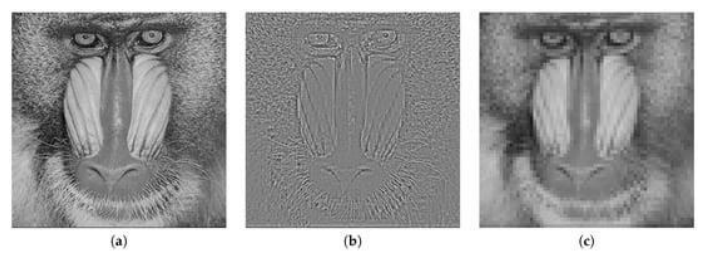
\includegraphics[scale=0.7]{graphics/chapter-2/chap2-dc-tinh-tinh.png}
    \caption{Hình ảnh JPEG tái xây dựng con tinh tinh bằng cách sử dụng các tập hợp khác nhau của các hệ số DCT đã được lượng tử hóa. }
    \label{fig:chap2-dc-tinh-tinh}
\end{figure}

\section{Brief Introduction to JPEG Baseline Encoding and Decoding}

Phần này tóm tắt ngắn gọn các bước mã hóa và giải mã cơ bản của JPEG để hỗ trợ việc hiểu về phương pháp đề xuất. JPEG là một kỹ thuật nén mất mát dựa trên khối, biến đổi các khối ảnh kích thước 8x8 thành các khối hệ số DCT đã được lượng tử hóa 8x8. Quá trình biến đổi bao gồm việc chuẩn hóa bằng cách trừ 128 từ mỗi pixel, biến đổi góc dọc disket (DCT), chia cho bảng lượng hóa, thường được tỉ lệ bằng một hệ số tỉ lệ gọi là hệ số lượng tử (QF) để kiểm soát hiệu ứng của nén và chất lượng hình ảnh sau đó làm tròn được để làm cho các giá trị trở thành số nguyên. 

DCT được định nghĩa như sau: 

\begin{equation}
\label{eq:chap2-DCT}
DCT_{u,v} = \frac{\alpha (u) \alpha (v)}{4} \sum _{i=0}^7 \sum_{j=0}^7 p_{i,j} \cos{[\frac{(2i + 1)u\pi}{16}]} \cos{ \frac{(2j + 1)v\pi}{16}}
\end{equation}
trong đó
\begin{equation}
\label{eq:chap2-DCT-condition}
\alpha(u) =
    \begin{cases}
        \frac{1}{\sqrt{2}} & $if u = 0$ \\
        1  & $if $ else 
    \end{cases}
\end{equation}

và $p_{i,j}$ đại diện cho giá trị pixel tại vị trí $(i,h), ĐCT_{u,v}$ tại vị trí $(u,v)$.

Sau khi thu được các hệ số DCT đã lượng tử hóa, chúng sẽ được nén có mất mát. Các hệ số DCT đã được lượng tử hóa bao gồm hệ số DC và hệ số AC đã được lượng tử hóa.  

Hệ số DC đã được lượng tử hóa là giá trị hệ số DCT đầu tiên và biểu thị một hình thức của giá trị pixel trung bình. Còn hệ số AC đã được lượng tử hóa là phần còn lại của các hệ số DCT và biểu thị các chi tiết tinh vi của khối pixel.


\textbf{Mã hoá mã xung hướng sai biệt} (DPCM - differential pulse code modulation), trong đó sự khác biệt giữa hai giá trị liên tiếp được mã hoá, được sử dụng để nén các hệ số DC đã được lượng tử hóa trong hai khối liền kề. Sau đó, các giá trị DPCM được nén mất mát bằng cách sử dụng một biến thể của mã hóa Huffman. Đối với các hệ số AC đã được lượng tử hóa, sẽ tiến hành mã hóa độ dài chuỗi, sau đó mã hóa bằng cách sử dụng một biến thể của mã hóa Huffman. 

Để tái tạo lại các pixel từ các hệ số DCT đã được lượng tử hóa, chúng ta nhân các hệ số DCT đã được lượng tử hóa với bảng lượng tử hóa và sau đó áp dụng biến đổi DCT ngược. Sau đó, chúng ta thêm 128 vào từng giá trị để hoàn ngược quá trình chuẩn hóa và cuối cùng, sử dụng hàm làm tròn để biến kết quả thành số nguyên. 

Thông tin chi tiết hơn về việc mã hóa và giải mã JPEG có thể được tìm thấy trong tài liệu ISO. Từ đây trở đi, các hệ số DCT đã được lượng tử hóa (bao gồm cả hệ số AC và hệ số DC đã được lượng tử hóa) sẽ được ký hiệu bằng chữ đậm: DCT, AC và DC. 

\section{Proposed Method}
Phương pháp đề xuất sử dụng một kỹ thuật ẩn dữ liệu có khả năng đảo ngược gọi là dịch chuyển biểu đồ tần số, trong đó hiệu suất phụ thuộc mạnh vào độ chính xác của dự đoán. Việc nhúng và sự méo mó của dịch chuyển biểu đồ tần số tương quan với lỗi dự đoán; lỗi dự đoán nhỏ hơn có nghĩa là khả năng nhúng cao hơn với méo mó thấp hơn. 

Các công trình trước đó không sử dụng các kỹ thuật dự đoán nâng cao trong việc ẩn dữ liệu có khả năng đảo ngược trong JPEG vì người ta nghĩ rằng việc dự đoán trong miền DCT là khá khó khăn và không đáng đối với công sức bỏ ra.  

Mặc dù giả định này đúng, nhưng không đúng cho tất cả DCT. DCT đầu tiên trong khối được0 biến đổi DCT, còn được gọi là hệ số DC. Phương pháp đề xuất xây dựng trên ý tưởng này để đề xuất một phương pháp dự đoán DC, sẽ tăng khả năng nhúng và giảm méo mó. 

\textbf{Hình \ref{fig:chap2-comparíon}} cho thấy biểu đồ tần số của hình ảnh Lena (QF = 50). Biểu đồ tần số của DC có nhiều đỉnh và có entropi lớn nhất, biểu đồ tần số của hệ số DC dự đoán khác biệt (DPCM) tốt hơn cho dịch chuyển biểu đồ tần số so với biểu đồ DC vì nó có một đỉnh cao xung quanh 0 và entropi thấp hơn, và cuối cùng, biểu đồ tần số của biểu đồ lỗi dự đoán DC đề xuất có đỉnh cao nhất và entropi nhỏ nhất, tạo nên lựa chọn lý tưởng cho việc dịch chuyển biểu đồ tần số. 

\begin{figure}
    \centering
    \includegraphics[scale=0.7]{graphics/chapter-2/chap2-comparíon.png}
    \caption{So sánh các biểu đồ tần số khác nhau. Biểu đồ lỗi dự đoán DC đề xuất có đỉnh cao nhất và entropi nhỏ nhất. (a) Biểu đồ tần số DC; (b) Biểu đồ tần số DPCM DC; (c) Biểu đồ lỗi dự đoán DC}
    \label{fig:chap2-comparíon}
\end{figure}

Các phần tiếp theo mô tả phương pháp dự đoán DC, phương pháp nhúng và phương pháp trích xuất. 

\subsection{DC Prediction}

Trong việc dự đoán trong nén hình ảnh, chỉ có các khối giải mã có thể được sử dụng cho dự đoán, dự đoán trong ẩn dữ liệu có khả năng đảo ngược có thể sử dụng tất cả các khối không được sử dụng để nhúng. Nói cách khác, chúng ta có thể chia các khối thành hai tập không chồng chéo, tập "trắng" và tập "đen", và nhúng chúng một lần để tạo điều kiện cho việc dự đoán chính xác hơn (xem \textbf{Hình \ref{fig:chap2-DCT-block}}). Không mất tính tổng quát, tập trắng được nhúng trước, sau đó tới tập đen. 

\begin{figure}
    \centering
    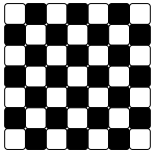
\includegraphics{graphics/chapter-2/chap2-DCT-block.png}
    \caption{Caption}
    \label{fig:chap2-DCT-block}
\end{figure}

Trước khi giải thích phương pháp dự đoán đề xuất, ta định nghĩa $T$ hoặc target block như là khối mà chúng ta muốn dự đoán hệ số $DC$. Hơn nữa, chỉ số trên $AC$ được sử dụng để biểu thị rằng khối được tái xây dựng chỉ sử dụng thành phần $AC$.

Sau đó $T^{AC}$ được sử dụng để biểu thị khối mục tiêu đã tái xây dựng một phần bằng cách chỉ sử dụng thành phần $AC$ từ khối mục tiêu (giá trị $DC$ được đặt là 0). Do DCT là một hàm tuyến tính, $T$ có thể được phân rã gần đúng như sau: 
\begin{equation}
\label{eq:chap2-DCT}
T \approx T^{AC} + DC \times \frac{Q_1}{8}
\end{equation}
trong đó $Q_1$  là giá trị lượng tử hóa được sử dụng để chia hệ số $DC$ để thu được $DC$, $DC \times \frac{Q_1}{8}$ biểu thị tác động của biến đổi DCT nghịch đảo lên DC.

Phương pháp dự đoán đề xuất sử dụng các khối lân cận và các khối tái xây dựng một phần bằng cách chỉ sử dụng thành phần AC. Các khối \textbf{DCT} lân cận được biến đổi thành các khối pixel của "Bắc", "Đông", "Nam" và "Tây" đầu tiên. 

\textbf{Hình \ref{fig:chap2-example-context}} cho thấy góc nhìn đồ họa về sự chia tách. Khu vực màu đỏ đại diện cho các phần của các khối lân cận gần khối mục tiêu nhất, và khu vực màu vàng đại diện cho các phần của khối mục tiêu gần khối lân cận nhất. 

\begin{equation}
\label{eq:chap2-pixel-red-yl}
Pixel_{red} \approx Pixel_{yellow}
\end{equation}

\begin{figure}
    \centering
    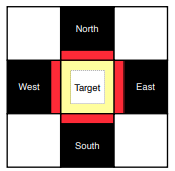
\includegraphics{graphics/chapter-2/chap2-example-context.png}
    \caption{Ví dụ về ngữ cảnh được sử dụng cho việc dự đoán.}
    \label{fig:chap2-example-context}
\end{figure}

\begin{figure}
    \centering
    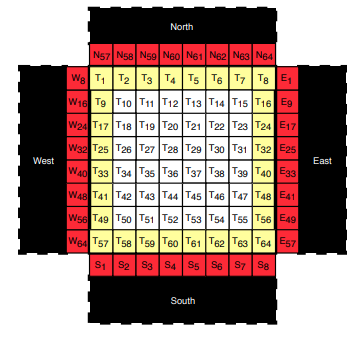
\includegraphics[scale=0.7]{graphics/chapter-2/chap2-example-context-predict-dc.png}
    \caption{Ngữ cảnh được sử dụng để dự đoán DC. Giá trị pixel láng giềng từ các khối đã giải mã (Bắc, Tây, Nam và Đông), và khối mục tiêu tái xây dựng một phần $T^{AC}$ được sử dụng để cải thiện độ chính xác dự đoán.}
    \label{fig:chap2-example-context-predict-dc}
\end{figure}

Kết hợp hai phương trình \ref{eq:chap2-DCT} và \ref{eq:chap2-pixel-red-yl}, ta có

\begin{equation}
\label{eq:apprro_pixel}
Pixel_{red} \approx Pixel_{yellow}^{AC} + DC \times \frac{Q_1}{8}
\end{equation}

Rút gọn lại phương trình, ta được \textbf{$\hat{DC}$}: là gá trị dự đoán của \textbf{DC}

\begin{equation}
\label{eq:appro_pixel_compact}
\textbf{$\hat{DC}$} = [\frac{8}{Q_1} \times (Pixel_{red} - Pixel_{yellow}^{AC}) ]
\end{equation}
với $[.]$ là hàm làm tròn số. Cuối cùng, vì có nhiều $Pixel_{red}$ và $Pixel_{yellow}^{AC}$ giá trị trung bình được sử dụng như một công cụ ước tính để đánh giá \textbf{$\hat{DC}$}:

\begin{equation}
\label{eq:DC_evaluation_1}
\textbf{$\hat{DC}$} = [\frac{8}{Q_1} \times \frac{\sum_{neighbor}(Pixel_{red} - Pixel_{yellow}^{AC})}{\# of neighhbors} ]
\end{equation}
\begin{equation}
\label{eq:DC_evaluation_2}
 = [\frac{8}{Q_1} \times \frac{\sum_{North, East, South, West}(Pixel_{red} - Pixel_{yellow}^{AC})}{32} ]
\end{equation}
\begin{equation}
\label{eq:DC_evaluation_3}
 = [\frac{8}{Q_1} \times \frac{\sum_{n=1}^8 (N_{56+n} - T_n^{AC}) + (E_{8n-7} - T_{8n}^{AC}) + (S_n - T_{n+56}^{AC}) + (W_{8n} - T_{8nn-7}^{AC})}{32} ]
\end{equation}


\subsection{Embedding}
Kỹ thuật dịch chuyển biểu đồ tần số được sử dụng để nhúng vào các giá trị lỗi dự đoán đã được nhúng được ký hiệu bằng $DC'$, và được thu được bằng cách sử dụng phương trình sau: 

\begin{equation}
\label{eq:DC_embeded}
DC'= \begin{cases}
$DC - b$ & $if  $  DC - \hat{DC} = - 1 \\
$DC + b$ & $if  $  DC - \hat{DC} = 0 \\
$DC - 1$ & $if  $  DC - \hat{DC} < -1 \\
$DC + 1$ & $if  $  DC - \hat{DC} > 0 \\
DC  & else
\end{cases}
\end{equation}

với $b \in \{0, 1\}$ là payload bit.

Kỹ thuật dịch chuyển biểu đồ tần số di chuyển DC với các sai số dự đoán nhỏ hơn -1 bằng -1, để có thể nhúng DC có giá trị -1 bằng cách sử dụng hệ số có giá trị -1 và -2: hệ số có giá trị -1 sẽ được thay đổi thành -2 nếu bit dữ liệu là "1", và giữ nguyên -1 nếu bit dữ liệu là "0". Logic tương tự áp dụng cho DC với sai số dự đoán lớn hơn 0. Vì kỹ thuật dịch chuyển biểu đồ tần số được áp dụng sao cho chúng không giao nhau, nên nó có thể được đảo ngược. Phần tiếp theo sẽ thảo luận về việc trích xuất dữ liệu và khôi phục lại  DC ban đầu.

\subsection{Extraction and Recovery}

Việc trích xuất dữ liệu và khôi phục lại DC ban đầu là khá đơn giản.

\begin{equation}
\label{eq:Extraction_1}
b= \begin{cases}
$0$ & $if  DC' = -1$ \\
$0$ & $if  DC' = 0$ \\
$1$ & $if  DC' = -2$ \\
$1$ & $if  DC' = 1$ \\
\end{cases}
\end{equation}

\begin{equation}
\label{eq:Extraction_2}
DC= \begin{cases}
$DC' + 1 $ & $ if $  DC' - \hat{DC} < 1 \\
$DC' - 1 $ & $ if  $  DC' - \hat{DC} > 0 \\
$DC'$ & $  if $ else\\
\end{cases}
\end{equation}

\section{Block Selection}

Việc lựa chọn khối là quan trọng trong các trường hợp không sử dụng hết khả năng nhúng đầy đủ. Để ảnh hưởng nhỏ nhất đến PSNR, các khối được sắp xếp theo độ mịn của chúng và các khối được nhúng tuần tự chỉ đến khi tất cả dữ liệu đã được nhúng. 

Để đảm bảo rằng các khối mịn nhất được nhúng trước, thuật toán lựa chọn khối được đề xuất bởi Huang et al. được sử dụng. Trong thuật toán này, số lượng hệ số DCT bằng 0 được sử dụng như một đại lượng đo độ mịn để sắp xếp các khối. Giả định ở đây là các khối DCT với nhiều hệ số DCT bằng không sẽ có ít chi tiết hơn và do đó mịn hơn. 

Trong phương pháp đề xuất, hệ số DCT bằng 0 không được sử dụng để đo độ mịn và chỉ các hệ số DCTbằng 0 được sử dụng để đo độ mịn. Hệ số DCT không được sử dụng vì chúng có thể thay đổi sau khi nhúng.

\section{Encoder and Decoder}
Phần này tóm tắt phương pháp mã hóa và giải mã của việc ẩn dữ liệu đảo ngược được đề xuất. Mỗi phần nhỏ sẽ mô tả các bước thực hiện và bao gồm các chi tiết thực hiện nhỏ để giúp hiểu rõ hơn. 

\subsection{Encoder}
\begin{enumerate}
    \item Trích xuất các khối DCT từ hình ảnh JPEG.
    \item Chia các khối thành tập trắng và tập đen. 
    \item Sử dụng phương pháp lựa chọn khối để sắp xếp tập trắng của DC
    \item Dự đoán tập trắng của  DC và nhúng nửa lượng dữ liệu nhúng.
    \item Sử dụng phương pháp lựa chọn khối để sắp xếp tập đen của DC.
    \item Dự đoán tập đen của DC và nhúng phần còn lại của dữ liệu nhúng bao gồm độ dài của dữ liệu nhúng, được thêm vào phía trước phần còn lại của dữ liệu nhúng. (Dự đoán sử dụng $DC'$ đã được nhúng từ bước 4.) 
\end{enumerate}

\subsection{Decoder}

\begin{enumerate}
    \item Trích xuất các khối DCT đã được nhúng từ hình ảnh JPEG. 
    \item Chia các khối thành tập trắng và tập đen.
    \item Sử dụng phương pháp lựa chọn khối để sắp xếp tập đen của $DC'$.
    \item Dự đoán tập đen của $DC'$, trích xuất độ dài của dữ liệu nhúng và nửa phần của dữ liệu nhúng, và khôi phục lại DC ban đầu cho tập đen.
    \item Sử dụng phương pháp lựa chọn khối để sắp xếp tập trắng của DC.
    \item Dự đoán tập trắng của $DC'$, trích xuất nửa đầu của dữ liệu nhúng, và khôi phục lại DC ban đầu cho tập trắng. (Dự đoán sử dụng DC ban đầu đã khôi phục từ bước 4.) 
\end{enumerate}

\section{Experiment}

Hiệu suất của phương pháp đề xuất được xác minh bằng cách sử dụng so sánh PSNR (giữa hình ảnh JPEG gốc và hình ảnh JPEG đã nhúng) và so sánh ưu điểm về kích thước tệp (do quá trình nhúng) của các phương pháp. Tuy nhiên, không có công trình nào hiện có tập trung vào việc nhúng trong DC. Do đó, một biến thể của phương pháp của Huang et al., là thuật toán tiên tiến nhất về PSNR và lợi ích về kích thước tệp, được so sánh với phương pháp đề xuất. 

Các giá trị của hệ số lượng tử hóa (QF) 50 và 80 được chọn để so sánh. Bảng lượng tử hóa dựa trên QF =50 là bảng lượng tử hóa cơ sở được khuyến nghị viết trong tài liệu tiêu chuẩn, được tỷ lệ để thu được bảng lượng tử hóa khác, là một bộ tiêu chuẩn tốt để kiểm tra. Bảng lượng tử hóa dựa trên QF =80 là bảng được biết đến là đạt được tỷ lệ nén tốt. 